\documentclass[10pt, aspectratio=169]{beamer}

% ─────────────────────────────────────────────────────────────────────────────
% Theme & Color Setup
% ─────────────────────────────────────────────────────────────────────────────
\usetheme{Madrid}
\usecolortheme{default}

\definecolor{PrimaryNavy}{RGB}{20, 35, 60}
\definecolor{AccentBlue}{RGB}{0, 114, 206}
\definecolor{TealAccent}{RGB}{0, 150, 166}
\definecolor{DarkRed}{RGB}{180, 40, 40}
\definecolor{CodeBg}{RGB}{245, 247, 250}
\definecolor{BlockBg}{RGB}{235, 240, 248}

\setbeamercolor{palette primary}{bg=PrimaryNavy,fg=white}
\setbeamercolor{palette secondary}{bg=AccentBlue,fg=white}
\setbeamercolor{palette tertiary}{bg=PrimaryNavy,fg=white}
\setbeamercolor{titlelike}{parent=palette primary,fg=white}
\setbeamercolor{frametitle}{bg=PrimaryNavy,fg=white}
\setbeamercolor{block title}{bg=PrimaryNavy,fg=white}
\setbeamercolor{block body}{bg=BlockBg,fg=black}
\setbeamercolor{block title example}{bg=TealAccent,fg=white}
\setbeamercolor{block body example}{bg=BlockBg,fg=black}
\setbeamercolor{block title alert}{bg=DarkRed,fg=white}
\setbeamercolor{block body alert}{bg=BlockBg,fg=black}

\setbeamertemplate{navigation symbols}{}
\setbeamertemplate{footline}[frame number]

% ─────────────────────────────────────────────────────────────────────────────
% Packages
% ─────────────────────────────────────────────────────────────────────────────
\usepackage{amsmath, amssymb}
\usepackage{booktabs}
\usepackage{multicol}
\usepackage{listings}
\usepackage{xcolor}
\usepackage{tikz}

% Code snippet styling
\lstset{
    language=Python,
    backgroundcolor=\color{CodeBg},
    basicstyle=\ttfamily\scriptsize,
    keywordstyle=\color{AccentBlue}\bfseries,
    stringstyle=\color{TealAccent},
    commentstyle=\color{gray}\itshape,
    breaklines=true,
    frame=single,
    rulecolor=\color{gray!30},
    showstringspaces=false
}

% ─────────────────────────────────────────────────────────────────────────────
% Title Slide Metadata
% ─────────────────────────────────────────────────────────────────────────────
\title[Consistency-Constrained Bengali Hate Speech MTL]{Consistency-Constrained Multi-Task Learning for Bengali Hate Speech Classification \& Generative Explanation}
\subtitle{6-Week Research Execution Plan, Smoke Testing Pipeline \& TigerLLM Benchmarking}
\author[Research Team]{Angkon \& Nahid \\ \small Senior Advisor Guidance Integrated}
\institute[ICCIT 2026]{Target Venue: ICCIT 2026 (Cox's Bazar) / IEEE Access}
\date{\today}

\begin{document}

% Slide 1: Title
\begin{frame}
    \titlepage
\end{frame}

% Slide 2: Executive Summary & Core Motivation
\begin{frame}{Executive Summary \& Core Motivation}
    \begin{columns}
        \begin{column}{0.5\textwidth}
            \begin{block}{The Core Challenge}
                \begin{itemize}
                    \item Online hate speech in Bengali is **multi-dimensional** (\textit{Hate Type}, \textit{Target}, \textit{Severity}).
                    \item Existing Multi-Task Models suffer from **logical inconsistency**:
                    \begin{itemize}
                        \item Predicting $\text{Type} = \text{None}$, but $\text{Target} = \text{Community}$.
                        \item Predicting $\text{Type} = \text{None}$, but $\text{Severity} = \text{Severe}$.
                    \end{itemize}
                    \item Existing explanation datasets (e.g., BanHADEX) **lack severity conditioning** and use incompatible taxonomies.
                \end{itemize}
            \end{block}
        \end{column}
        \begin{column}{0.5\textwidth}
            \begin{block}{Our Proposed Solution}
                \begin{itemize}
                    \item **Backbone**: Fine-tuned \texttt{csebuetnlp/banglabert} encoder.
                    \item **Multi-Task Heads**: 3 classification heads + 1 generative decoder head.
                    \item **Novel Loss ($\mathcal{L}_{\text{consist}}$)**: Differentiable soft penalty penalizing contradictory prediction vectors.
                    \item **Generative Explanations**: Conditioned on all 3 target labels using LLM Silver-Standard annotations.
                \end{itemize}
            \end{block}
        \end{column}
    \end{columns}
\end{frame}

% Slide 3: Taxonomy & Dataset Gap
\begin{frame}{Taxonomy Mapping \& Dataset Strategy}
    \begin{table}
        \centering
        \scriptsize
        \begin{tabular}{lp{4cm}p{4cm}}
            \toprule
            \textbf{Dimension} & \textbf{BanglaMultiHate (Primary ~50K)} & \textbf{BanHADEX (Reference ~19K)} \\
            \midrule
            \textbf{Hate Type} & Abusive, Sexism, Religious Hate, Political Hate, Profane, None & Political, Religious, Gender, Personal, Abusive, Origin, Body Shaming \\
            \textbf{Target} & Individual, Organization, Community, Society, None & 7 specific target groups \\
            \textbf{Severity} & Little to None, Mild, Severe & \textcolor{DarkRed}{\textbf{Not Present (Major Gap)}} \\
            \textbf{Explanations} & \textcolor{AccentBlue}{\textbf{Generated via Silver Pipeline (Gemini/TigerLLM)}} & Human-written (Unconditioned on severity) \\
            \bottomrule
        \end{tabular}
        \caption{Taxonomy schema comparison justifying Silver-Standard Explanation Generation.}
    \end{table}
    
    \begin{alertblock}{Key Research Takeaway}
        BanHADEX explanations cannot be directly reused because they lack severity conditioning. Therefore, we construct 5,000 Silver-Standard Bengali explanations conditioned on the full 3-task taxonomy.
    \end{alertblock}
\end{frame}

% Slide 4: Proposed Architecture
\begin{frame}{Model Architecture: Multi-Task + Consistency + Generation}
    \begin{center}
        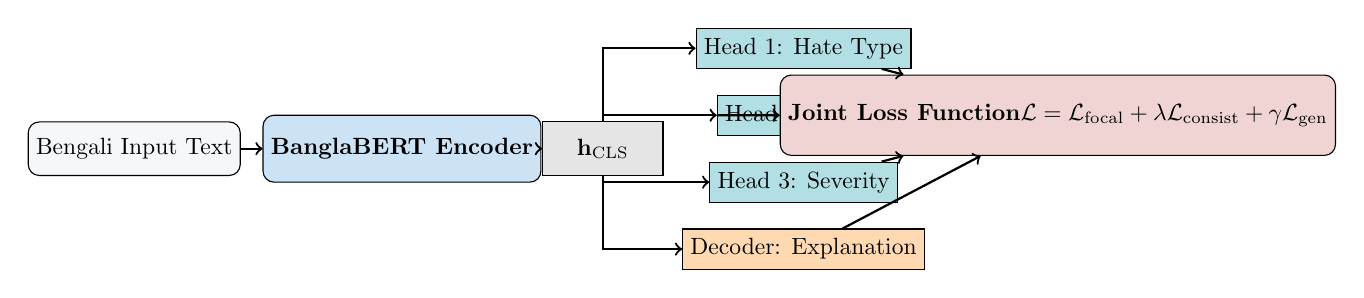
\begin{tikzpicture}[scale=0.85, every node/.style={transform shape}]
            % Input
            \node[draw, fill=CodeBg, minimum width=2.5cm, minimum height=0.8cm, rounded corners] (input) at (0,0) {Bengali Input Text};
            % Encoder
            \node[draw, fill=AccentBlue!20, minimum width=3.5cm, minimum height=1cm, rounded corners] (encoder) at (4,0) {\textbf{BanglaBERT Encoder}};
            % Dense Representation
            \node[draw, fill=gray!20, minimum width=1.8cm, minimum height=0.8cm] (cls) at (7,0) {$\mathbf{h}_{\text{CLS}}$};
            
            % Heads
            \node[draw, fill=TealAccent!30, minimum width=2.2cm, minimum height=0.6cm] (h1) at (10,1.5) {Head 1: Hate Type};
            \node[draw, fill=TealAccent!30, minimum width=2.2cm, minimum height=0.6cm] (h2) at (10,0.5) {Head 2: Target};
            \node[draw, fill=TealAccent!30, minimum width=2.2cm, minimum height=0.6cm] (h3) at (10,-0.5) {Head 3: Severity};
            \node[draw, fill=orange!30, minimum width=2.2cm, minimum height=0.6cm] (h4) at (10,-1.5) {Decoder: Explanation};
            
            % Loss
            \node[draw, fill=DarkRed!20, minimum width=3cm, minimum height=1.2cm, rounded corners] (loss) at (13.8,0.5) {\textbf{Joint Loss Function}\\$\mathcal{L} = \mathcal{L}_{\text{focal}} + \lambda \mathcal{L}_{\text{consist}} + \gamma \mathcal{L}_{\text{gen}}$};
            
            % Arrows
            \draw[->, thick] (input) -- (encoder);
            \draw[->, thick] (encoder) -- (cls);
            \draw[->, thick] (cls) |- (h1);
            \draw[->, thick] (cls) |- (h2);
            \draw[->, thick] (cls) |- (h3);
            \draw[->, thick] (cls) |- (h4);
            \draw[->, thick] (h1) -- (loss);
            \draw[->, thick] (h2) -- (loss);
            \draw[->, thick] (h3) -- (loss);
            \draw[->, thick] (h4) -- (loss);
        \end{tikzpicture}
    \end{center}
\end{frame}

% Slide 5: Mathematical Formulation
\begin{frame}{Mathematical Formulation: Soft Consistency Loss}
    \begin{block}{Logical Rules Enforced}
        \begin{enumerate}
            \item If $\text{Type} = \text{None} \implies \text{Target} = \text{None}$ AND $\text{Severity} = \text{Little to None}$.
            \item Contrapositive: If $\text{Target} \neq \text{None}$ OR $\text{Severity} \neq \text{Little to None} \implies \text{Type} \neq \text{None}$.
        \end{enumerate}
    \end{block}

    \begin{exampleblock}{Differentiable Consistency Loss ($\mathcal{L}_{\text{consist}}$)}
        Let $P_{\text{type}}(\text{None})$, $P_{\text{target}}(\neq \text{None})$, $P_{\text{sev}}(\neq \text{Little})$, and $P_{\text{sev}}(\text{Severe})$ be soft output probabilities:
        $$\mathcal{L}_{\text{consist}} = \frac{1}{N} \sum_{i=1}^{N} \left[ P_i(\text{type=None}) \cdot P_i(\text{target}\neq\text{None}) + P_i(\text{type=None}) \cdot P_i(\text{sev}\neq\text{Little}) + 2 \cdot P_i(\text{type=None}) \cdot P_i(\text{sev=Severe}) \right]$$
    \end{exampleblock}
    
    \begin{itemize}
        \item Fully differentiable formulation allows direct gradient backpropagation during fine-tuning.
        \item Dynamic weighting $\lambda(e)$ warms up linearly over epochs $e$.
    \end{itemize}
\end{frame}

% Slide 6: Senior's Guidance 1 — Mandatory Smoke Testing
\begin{frame}[fragile]{Senior's Guidance 1: Mandatory Pipeline Smoke Test}
    \begin{alertblock}{Why Senior Recommended Smoke Testing First}
        Running a **5-minute Smoke Test on 20 dummy samples** before generating 5,000 API explanations or launching 15-epoch training loops prevents wasted GPU time, API costs, or Colab crashes from tensor shape mismatches and loss NaNs.
    \end{alertblock}

    \begin{lstlisting}[language=Python]
# === smoke_test.py Snippet ===
import torch
from src.dataset import BanglaHateDataset
from src.model import ConsistencyConstrainedMTL
from src.losses import ConsistencyPenaltyLoss

# 1. Load dummy dataset (10 samples)
loader = torch.utils.data.DataLoader(BanglaHateDataset('data/dummy_smoke_test.csv'), batch_size=2)
batch = next(iter(loader))

# 2. Test forward pass & backpropagation
model = ConsistencyConstrainedMTL('csebuetnlp/banglabert')
optimizer = torch.optim.AdamW(model.parameters(), lr=1e-4)

type_out, target_out, sev_out, _ = model(batch['input_ids'], batch['attention_mask'])
loss = ConsistencyPenaltyLoss()(type_out, target_out, sev_out)
loss.backward()
optimizer.step()
print(f"Smoke Test Passed! Loss: {loss.item():.4f}")
    \end{lstlisting}
\end{frame}

% Slide 7: Senior's Guidance 2 — TigerLLM Integration
\begin{frame}{Senior's Guidance 2: TigerLLM Integration (ACL 2025)}
    \begin{columns}
        \begin{column}{0.5\textwidth}
            \begin{block}{What is TigerLLM?}
                \begin{itemize}
                    \item Open-source Bengali Large Language Model (\textbf{ACL 2025}, Raihan et al.).
                    \item Available in **1B and 9B** parameter sizes (\texttt{csebuetnlp/TigerLLM-9B}).
                    \item Instruction-tuned on \textbf{Bangla-Instruct} (100K high-quality pairs).
                \end{itemize}
            \end{block}

            \begin{block}{Role 1: Local Silver Generator}
                \begin{itemize}
                    \item Replaces/complements Gemini 1.5 Pro.
                    \item Runs locally on Kaggle/Colab GPU for **free** with zero rate limits.
                \end{itemize}
            \end{block}
        \end{column}

        \begin{column}{0.5\textwidth}
            \begin{block}{Role 2: SOTA Open-Source LLM Baseline}
                \begin{itemize}
                    \item Evaluated in zero-shot / few-shot mode on hate speech test set.
                    \item Answers reviewer critique: \textit{"Why fine-tune BanglaBERT instead of prompting a Bengali LLM?"}
                \end{itemize}
            \end{block}

            \begin{block}{Role 3: Automated Explanation Judge}
                \begin{itemize}
                    \item Serves as an LLM-as-a-judge to evaluate explanation quality and fluency.
                \end{itemize}
            \end{block}
        \end{column}
    \end{columns}
\end{frame}

% Slide 8: Experiment Matrix & Ablations
\begin{frame}{Experiment Matrix (4 BanglaBERT Ablations + 3 LLM Baselines)}
    \begin{table}
        \centering
        \scriptsize
        \begin{tabular}{llllp{4.5cm}}
            \toprule
            \textbf{Exp ID} & \textbf{Model Backbone} & \textbf{Consistency $\mathcal{L}_{\text{consist}}$} & \textbf{Gen Decoder $\mathcal{L}_{\text{gen}}$} & \textbf{Research Purpose} \\
            \midrule
            \texttt{exp0\_tiger} & TigerLLM-9B & --- & --- & SOTA Bengali LLM Baseline (Zero-Shot / Few-Shot) \\
            \texttt{exp0\_llama} & Llama-3.2-3B & --- & --- & Multilingual LLM Baseline (BLP-2025 style) \\
            \midrule
            \texttt{exp1\_base} & BanglaBERT & \textcolor{DarkRed}{\textbf{No}} & \textcolor{DarkRed}{\textbf{No}} & Standard MTL Baseline \\
            \texttt{exp2\_cons} & BanglaBERT & \textcolor{TealAccent}{\textbf{Yes}} & \textcolor{DarkRed}{\textbf{No}} & Isolate Consistency Penalty Contribution \\
            \texttt{exp3\_gen} & BanglaBERT & \textcolor{DarkRed}{\textbf{No}} & \textcolor{TealAccent}{\textbf{Yes}} & Isolate Explanation Generation Contribution \\
            \texttt{exp4\_full} & BanglaBERT & \textcolor{TealAccent}{\textbf{Yes}} & \textcolor{TealAccent}{\textbf{Yes}} & \textbf{Our Full Proposed Architecture} \\
            \bottomrule
        \end{tabular}
        \caption{Complete experimental setup to prove both classification and consistency gains.}
    \end{table}
\end{frame}

% Slide 9: Evaluation Metrics Strategy
\begin{frame}{Comprehensive Evaluation Strategy}
    \begin{columns}
        \begin{column}{0.33\textwidth}
            \begin{block}{1. Classification}
                \begin{itemize}
                    \item Macro $F_1$ per task:
                    \begin{itemize}
                        \item $F_1^{\text{Type}}$
                        \item $F_1^{\text{Target}}$
                        \item $F_1^{\text{Severity}}$
                    \end{itemize}
                    \item Average Macro $F_1$.
                    \end{itemize}
            \end{block}
        \end{column}

        \begin{column}{0.33\textwidth}
            \begin{block}{2. Consistency Violation}
                \begin{itemize}
                    \item **Consistency Violation Rate (CVR)**:
                    $$\text{CVR} = \frac{\text{Violating Predictions}}{\text{Total Predictions}} \times 100\%$$
                    \item Key Goal: Lower CVR without sacrificing Macro $F_1$.
                \end{itemize}
            \end{block}
        \end{column}

        \begin{column}{0.33\textwidth}
            \begin{block}{3. ERASER Faithfulness}
                \begin{itemize}
                    \item **Comprehensiveness ($\text{Comp} \uparrow$)**: Sufficiency drop when rationale removed.
                    \item **Sufficiency ($\text{Suff} \downarrow$)**: Prediction strength using rationale only.
                    \item **AOPC Score**.
                \end{itemize}
            \end{block}
        \end{column}
    \end{columns}
\end{frame}

% Slide 10: 6-Week Calendar Roadmap
\begin{frame}{6-Week Execution Roadmap}
    \begin{center}
        \small
        \begin{tabular}{cll}
            \toprule
            \textbf{Week} & \textbf{Timeline} & \textbf{Key Focus \& Deliverables} \\
            \midrule
            \textbf{Week 1} & Aug 19 -- Aug 25 & Environment Setup, EDA, Taxonomy Mapping \& \textbf{Pipeline Smoke Test} \\
            \textbf{Week 2} & Aug 26 -- Sep 01 & Silver Explanation Generation (Gemini 1.5 Pro + TigerLLM) \& Custom Data Scraping \\
            \textbf{Week 3} & Sep 02 -- Sep 08 & Model Architecture (\texttt{model.py}, \texttt{losses.py}) \& Custom Dataset Annotation \\
            \textbf{Week 4} & Sep 09 -- Sep 15 & Training 4 BanglaBERT Ablations + TigerLLM / Llama Baselines \\
            \textbf{Week 5} & Sep 16 -- Sep 22 & Evaluation (Classification $F_1$, CVR, ERASER Faithfulness Metrics) \\
            \textbf{Week 6} & Sep 23 -- Sep 30 & Paper Writing, High-Res Figures, Proofreading \& Final Submission \\
            \bottomrule
        \end{tabular}
    \end{center}
\end{frame}

% Slide 11: Task Division & Responsibilities
\begin{frame}{Team Task Division (Angkon \& Nahid)}
    \begin{table}
        \centering
        \small
        \begin{tabular}{lp{5.5cm}p{5.5cm}}
            \toprule
            \textbf{Phase} & \textbf{Angkon} & \textbf{Nahid} \\
            \midrule
            \textbf{Week 1} & Dataset Download \& Comprehensive EDA & Environment Setup, BanglaBERT \& \textbf{Smoke Test} \\
            \textbf{Week 2} & Silver Explanation Prompting (Gemini API) & TigerLLM Local Setup + Custom Scraping \\
            \textbf{Week 3} & Architecture Coding (\texttt{model.py}, \texttt{losses.py}) & Dataset Loader (\texttt{dataset.py}) + Annotation Lead \\
            \textbf{Week 4} & Run Ablations 1 \& 2 (\texttt{exp1}, \texttt{exp2}) & Run Ablations 3 \& 4 + LLM Baselines \\
            \textbf{Week 5} & Classification Metrics + CVR Analysis & ERASER Faithfulness Evaluation \\
            \textbf{Week 6} & Write §4-5 (Setup, Results \& Discussion) & Write §6-7 (Limitations, Conclusion, Figures) \\
            \bottomrule
        \end{tabular}
    \end{table}
\end{frame}

% Slide 12: Venue Strategy & Risk Mitigation
\begin{frame}{Venue Strategy \& Risk Management}
    \begin{columns}
        \begin{column}{0.5\textwidth}
            \begin{block}{Venue Options}
                \begin{itemize}
                    \item **Primary**: **ICCIT 2026** (Cox's Bazar, Dec 18-20). Deadline: Aug 31 / Extended Sep.
                    \item **Backup 1**: **IEEE Access** (Journal — Rolling deadline, high impact).
                    \item **Backup 2**: **BLP Workshop @ EMNLP 2027** (Top NLP venue).
                \end{itemize}
            \end{block}
        \end{column}

        \begin{column}{0.5\textwidth}
            \begin{block}{Risk Mitigation Plan}
                \begin{itemize}
                    \item **Compute OOM**: Use batch size 8 + gradient accumulation; optional \texttt{banglabert\_small}.
                    \item **API Rate Limits**: Checkpointing every 100 samples; fallback to local `TigerLLM-9B`.
                    \item **Trade-off Risk**: If $\mathcal{L}_{\text{consist}}$ drops $F_1$ slightly, CVR reduction remains a strong paper contribution.
                \end{itemize}
            \end{block}
        \end{column}
    \end{columns}
\end{frame}

% Slide 13: Summary & Immediate Next Steps
\begin{frame}{Summary \& Immediate Next Steps}
    \begin{alertblock}{Current Status}
        - Research design and mathematical loss formulation finalized.
        - Senior's feedback integrated (Smoke Testing + TigerLLM).
        - Workspace plan synchronized in \texttt{implementation\_plan2.md}.
    \end{alertblock}

    \begin{block}{Action Items for Today (Day 1)}
        \begin{enumerate}
            \item Execute \texttt{smoke\_test.py} on 10 dummy samples to verify PyTorch pipeline.
            \item Test \texttt{TigerLLM-9B} vs \texttt{Gemini 1.5 Pro} on 20 samples for Bengali explanation quality.
            \item Set up GitHub repository structure (\texttt{banglaHate/src}, \texttt{data}, \texttt{models}).
        \end{enumerate}
    \end{block}
    
    \begin{center}
        \Large \textbf{Thank You! Questions \& Feedback?}
    \end{center}
\end{frame}

\end{document}
